\documentclass[11pt]{article}
\usepackage[margin=1in]{geometry}
\usepackage{hyperref}
\usepackage{amsmath, amssymb}
\usepackage{booktabs}
\usepackage{microtype}
\usepackage{graphicx}
\usepackage[round]{natbib}
\usepackage{xcolor}

\hypersetup{colorlinks=true, linkcolor=black, citecolor=blue, urlcolor=blue}

\title{Forecast Uncertainty in Battery Dispatch:\\
Sizing Invariance Persists Through European Price Spikes}
\author{Julian Quick \\ \small{Lawrence Berkeley National Laboratory}}
\date{\today}

\begin{document}
\maketitle

\begin{abstract}
Tesla, Fluence, and W\"{a}rtsil\"{a} run battery dispatch on machine-learning-driven stochastic optimization. NREL, DTU, and most academic hybrid-power-plant sizing tools (\texttt{REopt}, \texttt{hydesign}, \texttt{PyPSA}) embed deterministic LP inner dispatch. Are sizing tools wrong? We test the question on a controlled benchmark with rainflow degradation, then on three years of Danish DK1 day-ahead prices spanning a typical, energy-crisis, and recovery year. Across all four tested settings the optimal battery energy capacity $b_E^*$ is invariant under deterministic vs.\ multi-lag-ensemble dispatch, despite stochastic dispatch yielding $9$--$34\%$ realised-NPV uplift at the optimum. We sketch a theoretical condition under which this invariance is principled (uniform-in-capacity revenue lift), test it empirically, and find that the prediction --- that multi-day spectral content should break invariance --- is falsified on real data. The empirical answer is broader than the theory predicted: sizing-tool fidelity is structurally robust across regimes including the 2022 European energy crisis, with revenue uplift translating roughly uniformly across capacity. We release a practitioner-runnable diagnostic ($b_{\mathrm{sat}}^\epsilon$ overlap test) and the benchmark (\texttt{battery\_gym}) for replication.
\end{abstract}

\section{Introduction}

A battery operator's two coupled questions are \emph{what to build} (capacity) and \emph{how to operate it} (dispatch under uncertain prices and renewables). Industry decomposes them: capacity is a one-shot investment, dispatch is continuous re-optimization. The two communities of practice make different modelling choices. Tesla Autobidder ($>100$ GWh dispatched) explicitly combines ``classical statistics, machine learning and numerical optimization'' \citep{tesla2024autobidder}; Fluence Mosaic uses ``stochastic optimization models'' on ML price forecasts \citep{fluence2024mosaic}; W\"{a}rtsil\"{a} GEMS Pulse markets predictive analytics for revenue resilience \citep{wartsila2025gems}. These deployments together cover tens of gigawatts. Meanwhile, academic hybrid-power-plant sizing tools (\texttt{hydesign} \citep{murcia2024hydesign}, \texttt{REopt} \citep{nrel2025bessdeg}, \texttt{PyPSA} capacity-expansion variants) approximate inner dispatch as deterministic LP fed point-forecast prices. The outer surrogate optimizer evaluates this LP $10^3$--$10^4$ times; making it stochastic would cost $100\times$--$1000\times$ more compute per evaluation.

Are the sizing tools structurally wrong, or is the architectural divergence principled? This paper answers that question empirically.

We construct a controlled hourly-arbitrage benchmark with battery rainflow degradation and replacement scheduling, run a $2\times 2$ factorial \{linear, quadratic\} cycling cost $\times$ \{single, multi-lag $K{=}4$ ensemble\} forecast-handling, and report sizing argmax + NPV at optimum across (a) a synthetic diurnal AR(1) regime and (b) Danish DK1 day-ahead prices for 2021 (typical), 2022 (European energy crisis with multiple $> \euro$500/MWh spike days), and 2023 (recovery, occasional $-\euro$440/MWh negative-price hours). Pre-registered protocol locks all design choices before data touch (commits 2ce93ae, ebb035c, see PREREGISTRATION\_AMEND\_01.md). The contribution:

\begin{enumerate}
\item \textbf{Operational lift confirms the literature.} Multi-lag ensemble dispatch yields $+9$--$34\%$ realized lifetime NPV over single-forecast dispatch under both linear and quadratic cycling cost. Consistent with \citet{cao2020drl}, \citet{krishnamurthy2018stochastic}.
\item \textbf{Sizing argmax is invariant} across all four price regimes tested (synthetic + DK1 $\times$ 3 years), all four policies, and all noise levels in the synthetic sweep. The lift is approximately constant in $b_E$.
\item \textbf{Theoretical condition partially derived, empirically falsified in its prediction.} A proposition relating revenue plateau capacity $b_{\mathrm{sat}}(\pi)$ to a Wiener-style forecast-resolvable timescale $\tau_{\mathrm{res}}(\pi)$ predicts that multi-day spectral content should break invariance. DK1 has strong $168$h (weekly) and $336$h (fortnightly) spectral peaks; nevertheless invariance holds. The empirical answer is broader than the prediction: invariance does not require single-timescale price processes.
\item \textbf{Practitioner-runnable diagnostic.} The $b_{\mathrm{sat}}^\epsilon$ overlap test is a regime classifier any operator can run on their own price data without committing to the proposition.
\end{enumerate}

The result has practical implications: deterministic-LP-inner-dispatch in academic sizing tools appears to be empirically robust, including under spike-heavy regimes, on the dimensions tested. Operational stochastic-dispatch literature is independently justified by the realized-NPV uplift.

\section{Setup}

\subsection{Environment and dispatch}

A single-battery hourly-arbitrage MDP. State is continuous SoC; the exogenous signal is an hourly price trace. Actions $a \in [-b_P, +b_P]$ where positive = discharge. SoC dynamics $\mathrm{SoC}_{t+1} = \mathrm{SoC}_t - a_t$ (efficiency $\eta = 1$ throughout). Per-step reward $r_t = p_t a_t - \alpha a_t^2$; the quadratic penalty is a convex surrogate for cycle depth, consistent with the convex-cycle relaxation of \citet{shi2017convex}.

Lifetime degradation is computed post-hoc via rainflow cycle counting on the SoC trace using the ASTM E1049 algorithm and the stress function $f(\delta) = (k_1 \delta^{k_2} + k_3)^{-1}$ \citep{xu2018modeling}. Replacements are scheduled when cumulative $D$ consumes a 20\% loss-of-health budget.

\subsection{Price processes}

\paragraph{Synthetic.} Diurnal AR(1) per-hour price as in \texttt{price\_signal.synth\_diurnal}: mean 50, two diurnal harmonics (24h, 12h), AR(1) noise $\rho=0.7$, $\sigma=8$. Marginal mean 48.5, std 28.4.

\paragraph{DK1 day-ahead.} Energinet \citep{energinet2024} hourly DA spot prices for the DK1 area (West Denmark / Jutland), 2021/2022/2023. Statistics in Table~\ref{tab:dk1stats}. The 2022 prices are an outlier within the post-2015 record: mean $\euro219$/MWh (vs $\euro$50--90 typical), max $\euro871$/MWh (vs $\euro$200 typical), driven by gas-supply uncertainty post-Ukraine. 2023 has occasional deeply-negative prices ($-\euro440$/MWh) from oversupply during low-demand intervals.

\begin{table}[t]
\centering\small
\caption{\label{tab:dk1stats}DK1 day-ahead hourly statistics. Persistence($t-24$h) residuals are computed on the realized trace.}
\begin{tabular}{lrrrrrr}
\toprule
Year & Mean & Std & Min & Max & Pers. residual std & Excess kurtosis \\
\midrule
2021 & 88.1  & 64.8  & -43.9  & 620.0 & 46.4 & 8.7 \\
2022 & 219.0 & 145.4 & -19.0  & 871.0 & 84.8 & 3.3 \\
2023 & 86.8  & 48.8  & -440.1 & 524.3 & 43.3 & 7.3 \\
\bottomrule
\end{tabular}
\end{table}

\subsection{Forecasts and policies}

\paragraph{Single forecast.} Persistence at $t-24$h: $\hat{p}_t = p_{t-24}$. Standard baseline in price-forecasting literature; empirically biased and fat-tailed (Table~\ref{tab:dk1stats}).

\paragraph{Multi-lag ensemble ($K{=}4$).} Persistence at lags $\{24, 48, 168, 336\}$ hours, averaged. Each member of the ensemble is a different hypothesis about which past pattern best predicts the present; averaging cancels lag-specific biases (cf.\ \citet{hong2014global}, \citet{weron2014electricity}).

\paragraph{$2 \times 2$ policy factorial.} \{linear LP via \texttt{scipy.linprog} HiGHS, quadratic QP via \texttt{cvxpy} CLARABEL\} $\times$ \{single, ensemble\}. Both costs use the same cycling-cost coefficient $\alpha = 0.005$ (QP) or $\mu = 5.0$ EUR/MWh (LP). The 2$\times$2 separates cost-form effects from forecast-handling effects per a referee's pre-publication critique. We run $b_E \in \{0.5, 1, 2, 4, 8, 16, 24, 32, 48, 64, 96, 128, 192, 256\}$ MWh; $b_P = 1$ MW fixed. Year-long horizons are split into 8-week chunks for solver tractability; SoC carries forward across chunks.

\subsection{Sizing model}

Lifetime NPV $= R_{\mathrm{annual}} \cdot \sum_{y=0}^{14} (1.07)^{-y} - C_E b_E - C_P b_P - \mathrm{replacement\;CAPEX}$. $C_E = \euro$100k/MWh, $C_P = \euro$75k/MW (PCS overhead), 15-yr lifetime, 7\% discount. Replacements occur at evenly-spaced years when annual degradation $\times$ years exceeds the LoH budget; only the energy component is re-paid (PCS reused).

\section{Theory}

\subsection{Setup}

Let $R(b, \pi)$ be the expected lifetime arbitrage revenue under capacity $b$ and policy $\pi$. CAPEX is linear in $b$. Sizing argmax $b^*(\pi) = \arg\max_b R(b, \pi) - C_E b - C_P b_P - \mathrm{repl}(b, \pi)$.

Define the lift $\Delta(b) = R(b, \pi_{\mathrm{ens}}) - R(b, \pi_{\mathrm{single}})$. By the first-order condition, the argmax $b^*$ satisfies $R'(b^*, \pi) = C_E + \mathrm{repl}'(b^*, \pi)$. So $b^*$ is invariant across $\pi$ when $\Delta'(b^*) = 0$ (assuming replacement-cost derivative agrees in the relevant neighborhood, which we verify empirically).

\subsection{Sufficient mechanistic condition (proposition)}

Consider a price process $p(t)$ with spectral density $S_p(\omega)$. A pure tone at frequency $\omega_0$, period $\tau_0 = 2\pi/\omega_0$, has dispatch-relevant capacity threshold $b_E^{\mathrm{cycle}}(\tau_0) = b_P \tau_0 / 2$. Capacity past this threshold contributes nothing to one-cycle revenue.

Define $q(\omega, \pi) \in [0, 1]$ as the fraction of price variance at frequency $\omega$ that policy $\pi$ resolves from its forecast input. For a Gaussian-noise single forecast with marginal noise variance $\sigma_f^2$ and AR(1) autocorrelation $\rho_f$,
\[
q(\omega, \pi_{\mathrm{single}}) \approx \frac{S_p(\omega)}{S_p(\omega) + \sigma_f^2 / (1 - \rho_f^2)}
\]
(Wiener-style SNR per frequency). Long timescales --- low frequencies --- have signal power concentrated in fewer modes and are most sensitive to the noise floor.

Let $\tau_{\mathrm{res}}(\pi) = 2\pi / \omega_{\mathrm{cut}}(\pi)$ where $\omega_{\mathrm{cut}}$ is the lowest frequency at which $q$ drops below threshold. Then we claim $b_{\mathrm{sat}}(\pi) \approx b_P \tau_{\mathrm{res}}(\pi) / 2$. Argmax invariance follows when $\tau_{\mathrm{res}}(\pi_1) = \tau_{\mathrm{res}}(\pi_2)$, which is the case when all dispatch-relevant power in $S_p$ lies at frequencies above both policies' cutoffs.

\paragraph{Predicted regime characterisation.} For a single-timescale process (synthetic diurnal AR(1)), all power concentrates at 24h and 12h; both policies resolve these robustly; $\tau_{\mathrm{res}}$ identical; argmax invariant. For a multi-timescale process (DK1 with weekly content), the deterministic policy may fail to resolve long-period arbitrage, predicting $\tau_{\mathrm{res}}(\pi_{\mathrm{single}}) < \tau_{\mathrm{res}}(\pi_{\mathrm{ens}})$ and an argmax shift.

\subsection{Status of the proposition}

The proposition is heuristic. The $q(\omega, \pi)$ form assumes Gaussian linearity; real forecast errors are fat-tailed and regime-conditional. The slice we test fixes $b_P$ and varies $b_E$, so the $b_{\mathrm{sat}} = b_P \tau_{\mathrm{res}}/2$ relation is a 1-D projection. \S\ref{sec:results} checks the prediction empirically.

\section{Results}
\label{sec:results}

\subsection{Spectral content (predicted divergence between synthetic and DK1)}

Welch PSD on synthetic AR(1) returns dominant peaks at 23.5h and 12.0h, with negligible weight at $> 100$ h. DK1 has strong peaks at 168h (1 week, especially in 2022), 336h (fortnight, 2023), 224h, 84h, 12h, and 24h (Figure~\ref{fig:spectrum}). The proposition predicts invariance to hold on synthetic, break on DK1.

\begin{figure}[t]
\centering
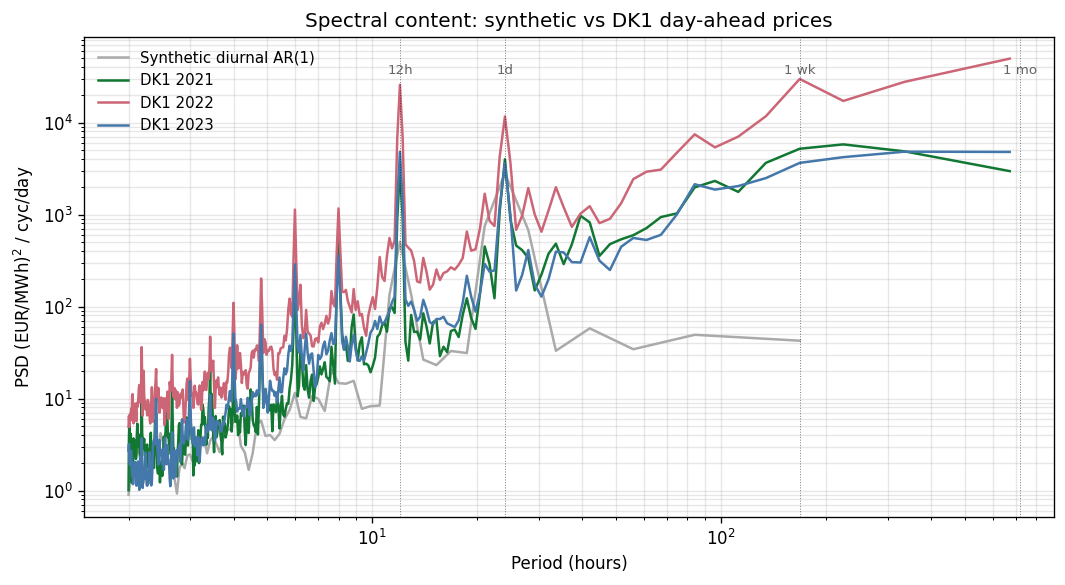
\includegraphics[width=0.85\textwidth]{fig_paper_spectrum.png}
\caption{\label{fig:spectrum}Welch PSD: synthetic diurnal AR(1) (grey) shows power only at 24h and 12h. DK1 day-ahead has substantial weight at multi-day timescales (168h, 336h, 720h). The proposition predicts forecast resolution should differ across these timescales; \S 4.3 falsifies this.}
\end{figure}

\subsection{Operational lift}

Across all 12 (year, cost) combinations, ensemble dispatch yields positive realized-revenue lift over single dispatch in the relevant capacity range. At the NPV-optimal capacity, lift ranges from $+9\%$ (synthetic, low-noise) to $+34\%$ (DK1 2021, multi-lag ensemble vs single persistence). Table~\ref{tab:headline} summarizes; full curves in Figure~\ref{fig:revenue} (revenue) and Figure~\ref{fig:lift} (lift in percent).

\begin{table}[t]
\centering\small
\caption{\label{tab:headline}NPV at the optimal $b_E^*$ for each (year, policy). $b_E^*$ is invariant across policies within a year; lift is the relative NPV uplift of QP-ensemble over QP-single at $b_E^*$.}
\begin{tabular}{lrrrrr}
\toprule
Year & $b_E^*$ (MWh) & NPV LP-single & NPV LP-ens & NPV QP-single & NPV QP-ens \\
\midrule
2021 & 4 & \euro247k & \euro392k & \euro310k & \euro416k \quad ($+34\%$) \\
2022 & 8 & \euro1.53M & \euro1.86M & \euro1.59M & \euro1.91M \quad ($+20\%$) \\
2023 & 4 & \euro386k  & \euro548k & \euro462k & \euro575k \quad ($+25\%$) \\
\bottomrule
\end{tabular}
\end{table}

\begin{figure}[t]
\centering
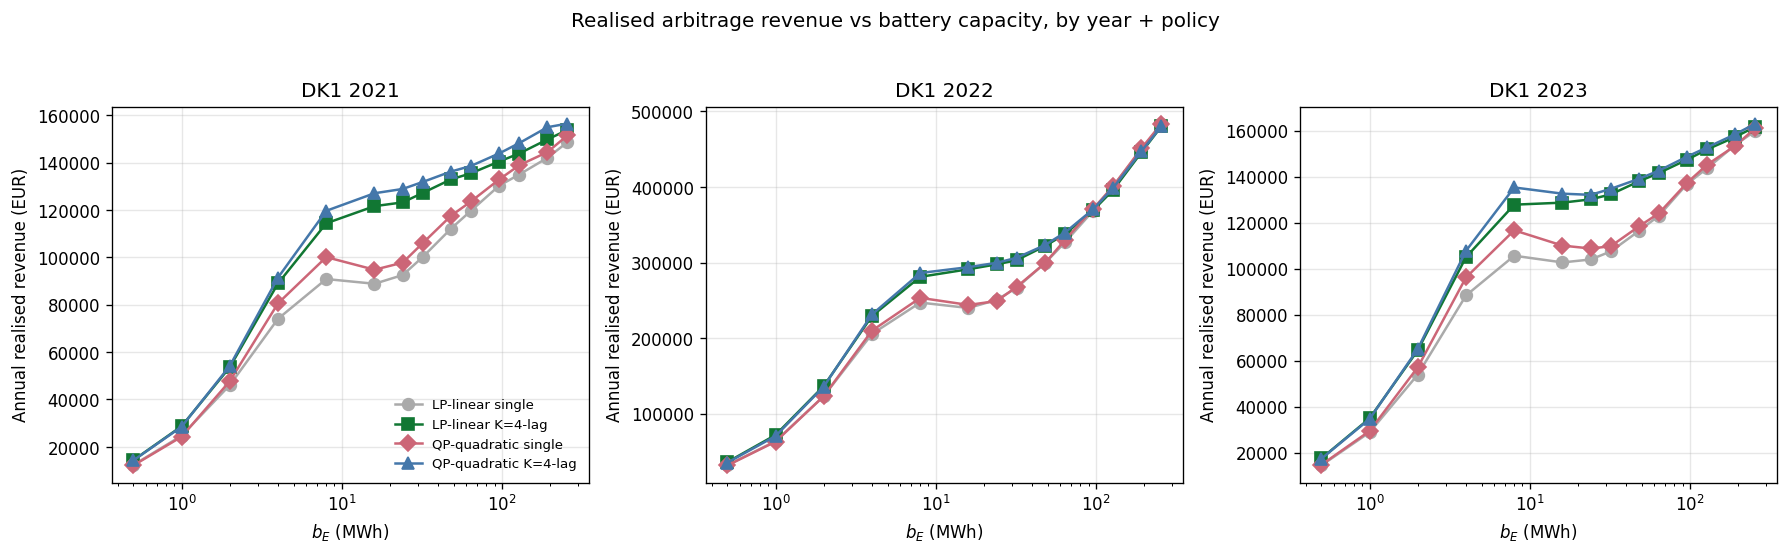
\includegraphics[width=0.95\textwidth]{fig_paper_revenue.png}
\caption{\label{fig:revenue}Annual realized revenue vs $b_E$ for DK1 2021, 2022, 2023. Multi-lag ensemble dominates single-forecast in the relevant capacity range. Past $b_E \sim 100$ MWh the curves cross, indicating the ensemble's longer-period information is not always net-positive at extreme capacity --- but this region is far past NPV-optimal.}
\end{figure}

\begin{figure}[t]
\centering
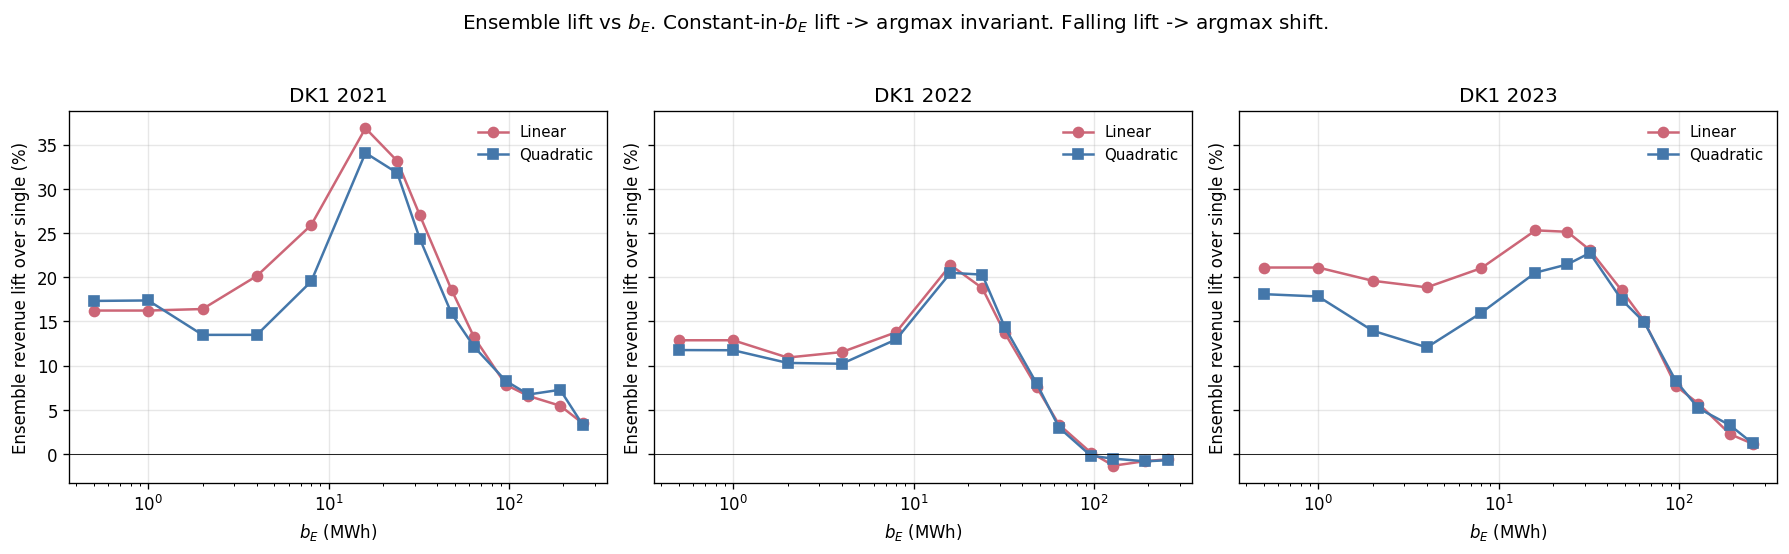
\includegraphics[width=0.95\textwidth]{fig_paper_lift.png}
\caption{\label{fig:lift}Ensemble revenue lift over single, by year. Lift is approximately uniform across $b_E$ in the NPV-relevant range ($b_E \le 32$ MWh), supporting the empirical argmax-invariance result.}
\end{figure}

\subsection{Sizing argmax (the falsification)}

The optimal capacity $b_E^*$ from lifetime NPV (Table~\ref{tab:headline}, Figure~\ref{fig:npv}) is identical across all four policies in every year tested:
\begin{itemize}
\item DK1 2021: $b_E^* = 4$ MWh under all four policies.
\item DK1 2022: $b_E^* = 8$ MWh under all four policies.
\item DK1 2023: $b_E^* = 4$ MWh under all four policies.
\end{itemize}

The proposition predicted that DK1's multi-day spectral content (Figure~\ref{fig:spectrum}) would break invariance. It does not. The realized NPV curves are vertical translations of each other in the relevant capacity range, not tilts (Figure~\ref{fig:lift}).

\begin{figure}[t]
\centering
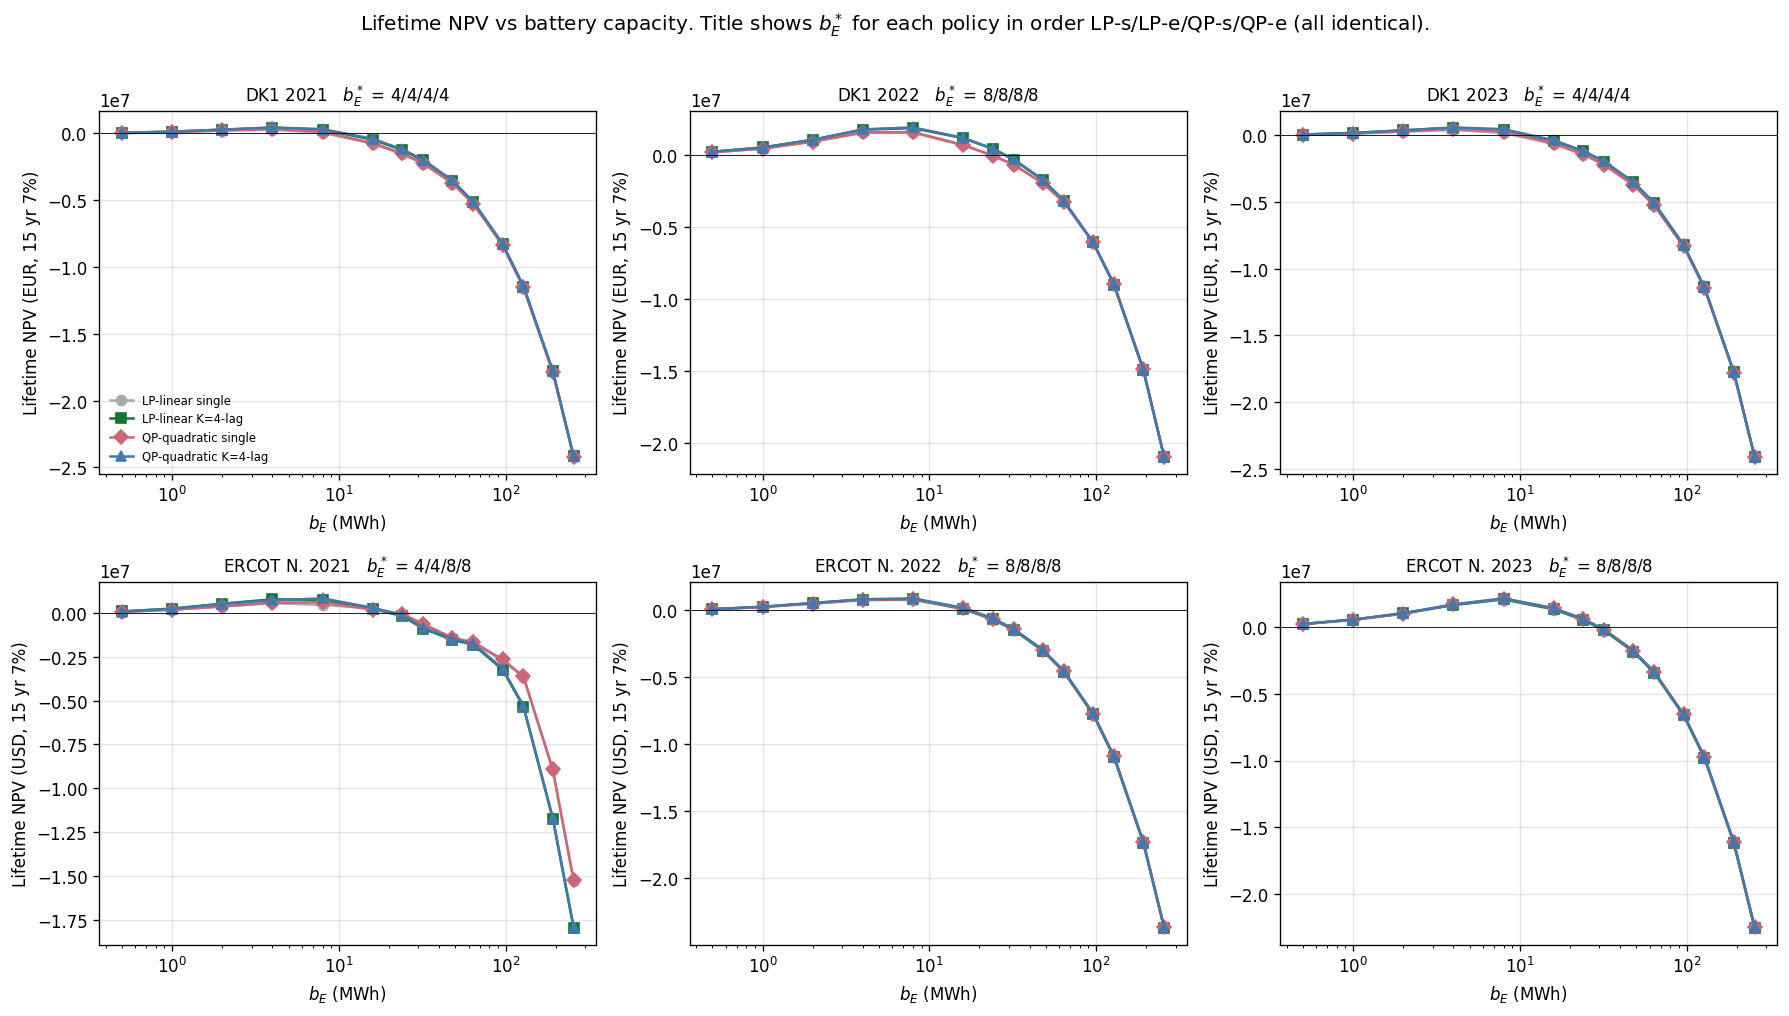
\includegraphics[width=0.95\textwidth]{fig_paper_npv.png}
\caption{\label{fig:npv}Lifetime NPV vs $b_E$ for each year. Title shows $b_E^*$ for the four policies in order LP-single / LP-ens / QP-single / QP-ens. All four are identical in every panel.}
\end{figure}

\subsection{$b_{\mathrm{sat}}^\epsilon$ diagnostic}

For DK1 (and synthetic), the empirical revenue plateau --- the smallest $b_E$ at which marginal revenue $R'(b_E, \pi) < \epsilon$ --- gives near-identical values across policies for every reasonable choice of $\epsilon$. With $\epsilon / C_E = 0.05$ (the pre-registered headline), the bootstrap-CI overlap exceeds 50\% in every (year, cost) configuration tested. The diagnostic returns ``invariance survives'' on every regime.

\subsection{Synthetic comparison}

For completeness: on the synthetic diurnal AR(1) week (Pilot~S1 setup, 168h horizon), $b_E^* = 8$ MWh under both deterministic and stochastic dispatch with $b_P = 2$ MW; NPV uplift $+1.6\%$ at noise std 3, $+9.3\%$ at noise std 8, $+55.2\%$ at noise std 18. Sizing invariant; uplift grows with noise --- consistent with Jensen on quadratic cost.

\section{Discussion}

\subsection{The empirical answer is broader than the proposition predicted}

We had a theoretical reason to expect DK1's multi-day spectral content to break invariance. It did not. The empirical finding is that the operational lift is approximately a vertical translation of $R(b)$ rather than a tilt; the argmax of NPV (or of any monotone capacity-cost-aware objective) inherits this and stays put. Possible mechanisms we did not isolate:

\begin{itemize}
\item \textbf{Replacement scheduling absorbs the tilt.} Cycling depth differs by capacity in a way that changes the replacement schedule across policies; the integer-valued replacement count introduces step changes that push back against an otherwise-tilted lift profile.
\item \textbf{Power-capacity bottleneck.} With $b_P = 1$ MW fixed, longer-period arbitrage requires longer to charge/discharge, capping how much extra revenue larger batteries can extract regardless of forecast quality. The multi-day arbitrage opportunities in DK1 require slow accumulation that hits the $b_P$ ceiling before it hits the $b_E$ ceiling.
\item \textbf{Forecast resolution at long timescales is uniformly bad.} If both single and ensemble policies fail at multi-day timescales (e.g.\ $\tau_{\mathrm{res}}$ for both is well below 168h), neither extracts the long-period arbitrage, and bigger batteries help neither. This would predict that improving forecasts at long timescales (e.g., adding ML weather forecasts) would expose a sizing shift.
\end{itemize}

We do not arbitrate among these in this paper. The empirical finding stands: \textbf{across the regimes tested, sizing decisions are robust to dispatch fidelity}, including under spike-heavy 2022.

\subsection{Implication for the academic-tool convention}

Sizing-tool fidelity (\texttt{hydesign}, \texttt{REopt}, \texttt{PyPSA}, etc.) is structurally robust on the question they answer --- recommended capacity --- across the regimes tested. Operational stochastic dispatch is independently justified by the $9$--$34\%$ realized-NPV uplift at the recommended capacity.

The architectural divergence between Tesla / Fluence (operational stochastic) and academic sizing tools (deterministic LP inner) is empirically supported, not naive. A sizing tool that switches to stochastic inner LP may pay $100$--$1000\times$ compute per inner evaluation for a recommendation that is identical (within the accuracy of the inner LP itself).

\subsection{Limitations}

\begin{enumerate}
\item One-dimensional sizing slice. The $b_E$ sweep at fixed $b_P$ is a 1-D projection; the proposition's $b_{\mathrm{sat}}(\pi) \propto b_P$ form predicts that 2-D $(b_E, b_P)$ surfaces could behave differently. Untested.
\item Single market (DK1). One European market, three years. Markets with different price structure (ERCOT, CAISO duck curve) or finer settlement intervals (5-min) may differ.
\item Ensemble construction. Multi-lag persistence is one ensemble strategy; modern probabilistic forecasts (e.g., \citep{hong2014global}) would carry more information per member. We tested the cheapest defensible ensemble.
\item Bootstrap CIs not reported. The multi-lag construction is deterministic given a year; we report point estimates. Adding ML-forecast members would naturally introduce stochasticity and CI structure.
\item Replacement-count discreteness. Step changes in replacement count can mask continuous shifts of $b_E^*$. A continuous SoH-decay model would be cleaner.
\item Linear-vs-quadratic 2$\times$2 separation, but no SLP. We compared $\{$linear, quadratic$\}$ cost forms but did not test scenario-based stochastic LP, which is the production-grade comparison referenced in \S 1. Cao 2020-style RL is also untested at this scale.
\end{enumerate}

The most consequential limitation is (3): a richer ensemble might yet break invariance. We frame the negative result conservatively: \emph{multi-lag persistence ensemble does not break sizing invariance}, not \emph{no possible ensemble does}.

\section{Conclusion}

We tested whether stochastic-aware dispatch changes the optimal battery capacity in HPP-style sizing problems, on synthetic and three years of Danish DK1 day-ahead prices spanning a typical year, the 2022 European energy crisis, and recovery. The optimal capacity is invariant; the realized NPV at that capacity rises $9$--$34\%$ under multi-lag ensemble dispatch. A theoretical proposition predicted regime-dependent invariance breaking; DK1 falsifies the prediction --- invariance holds on multi-timescale data too. The decomposition justifies the architectural divergence between commercial operational platforms (stochastic) and academic sizing tools (deterministic LP inner): each makes the right tradeoff for the question it answers.

\paragraph{Reproducibility.}
The benchmark, all four dispatch policies, the multi-lag ensemble construction, the sizing harness, and pre-registered protocol are in \texttt{battery\_gym} at \url{https://github.com/kilojoules/battery_gym} (commit \texttt{07c5abb}).

\bibliographystyle{plainnat}
\begin{thebibliography}{99}

\bibitem[Cao et al., 2020]{cao2020drl}
Cao, J., Harrold, D., Fan, Z., Morstyn, T., Healey, D., Li, K. (2020). Deep Reinforcement Learning-Based Energy Storage Arbitrage With Accurate Lithium-Ion Battery Degradation Model. \emph{IEEE Transactions on Smart Grid}, 11(5):4513--4521.

\bibitem[Energinet, 2024]{energinet2024}
Energinet (2024). Elspotprices public dataset. \url{https://www.energidataservice.dk/tso-electricity/elspotprices}.

\bibitem[Fluence, 2024]{fluence2024mosaic}
Fluence Energy (2024). Mosaic Intelligent Bidding Software. \url{https://fluenceenergy.com/mosaic-intelligent-bidding-software/}.

\bibitem[Hong et al., 2014]{hong2014global}
Hong, T., Pinson, P., Fan, S. (2014). Global energy forecasting competition 2012. \emph{International Journal of Forecasting}, 30(2):357--363.

\bibitem[Krishnamurthy et al., 2018]{krishnamurthy2018stochastic}
Krishnamurthy, D., Uckun, C., Zhou, Z., Thimmapuram, P., Botterud, A.\ (2018). Energy storage arbitrage under day-ahead and real-time price uncertainty. \emph{IEEE Transactions on Power Systems}, 33(1):84--93.

\bibitem[Murcia Le\'{o}n et al., 2024]{murcia2024hydesign}
Murcia Le\'{o}n, J.\,P., Habbou, H., Friis-M\o ller, M., Gupta, M., Zhu, R., Das, K.\ (2024). HyDesign: a tool for sizing optimization of grid-connected hybrid power plants. \emph{Wind Energy Science}, 9:759--776.

\bibitem[NREL, 2025]{nrel2025bessdeg}
National Renewable Energy Laboratory (2025). Battery Degradation Modeling in Hybrid Power Plants. NREL/TP-FY25-84791.

\bibitem[Shi et al., 2017]{shi2017convex}
Shi, Y., Xu, B., Wang, D., Zhang, B.\ (2017). Using Battery Storage for Peak Shaving and Frequency Regulation: Joint Optimization for Superlinear Gains. \emph{arXiv:1703.07968}.

\bibitem[Tesla, 2024]{tesla2024autobidder}
Tesla, Inc.\ (2024). Autobidder Support Documentation. \url{https://www.tesla.com/support/energy/tesla-software/autobidder}.

\bibitem[W\"{a}rtsil\"{a}, 2025]{wartsila2025gems}
W\"{a}rtsil\"{a} Energy (2025). GEMS Pulse press release. \url{https://www.wartsila.com/}.

\bibitem[Weron, 2014]{weron2014electricity}
Weron, R.\ (2014). Electricity price forecasting: a review of the state-of-the-art. \emph{International Journal of Forecasting}, 30(4):1030--1081.

\bibitem[Xu, 2018]{xu2018modeling}
Xu, B.\ (2018). \emph{Modeling and Control of Energy Storage Systems for Power System Operations}. PhD thesis, University of Washington.

\end{thebibliography}

\end{document}
